\chapter{Grant Mitt: Concentration Before Diversification}

This interview is not a physics lecture, but it has a spine that can be written with the same care we would give to a technical argument. Grant Mitt's claims form a compact model of commercial judgment: the market decides, most businesses are not exceptional economic bets, one concentrated engine usually creates the first large pile, distribution can arrive through personal credibility, and scale requires people who can execute fundamentals without the founder standing over them.

\section{The Market Does Not Care How Old You Are}

The interview begins with a young-founder problem. The question is not abstract confidence, but confidence in a market where the other owners may be two or three times older. Mitt's first move is to strip age of special status. If we make age the issue, he says, others will make it the issue. If we do not, the market has a simpler test.

In his analogy, business is like entering the NFL. A rookie and a nineteen-year veteran can both get cut. A rookie and a veteran can both win. The point is not that experience is irrelevant; the point is that the competitive arena eventually asks for performance.

We can write the market test schematically as
\begin{equation}
\text{Customer choice} = f(\text{trust},\text{offer},\text{execution},\text{price},\text{timing}),
\end{equation}
with age appearing only if the seller or the buyer makes it part of trust. In Mitt's telling, the market is not a committee awarding status. It is a selection mechanism.

\begin{remark}
The equation is not stated in the interview. It is a compact reconstruction of the argument: age is not the primitive variable; the transaction is.
\end{remark}

That sets up the next question. If the market is that unforgiving, why choose entrepreneurship at all?

\section{The Bad Base Rates Of Starting}

The next movement is important because it prevents the interview from becoming easy founder mythology. Mitt does not say that everyone should start a business. He first gives the base-rate warning.

According to the interview, about
\begin{equation}
P(\text{break even or lose money}) \approx 0.86,
\end{equation}
and only about
\begin{equation}
P(R_{\text{business}} > \$10{,}000{,}000) \approx 0.005.
\end{equation}
He then compares average income for employees and business operators, giving the rough shorthand
\begin{equation}
I_{\text{employee}} \approx \$58{,}000,\qquad
I_{\text{operator}} \approx \$55{,}000,
\end{equation}
or
\begin{equation}
I_{\text{employee}} - I_{\text{operator}}
\approx \$3{,}000\text{ to }\$4{,}000.
\end{equation}

These are interview claims, not audited statistical findings in these notes. Their role is structural. They make the obstacle explicit: starting a business is not automatically the rational path if the only question is average income.

\subsection{Question \& Answer}

\paragraph{Question.}
If most businesses break even, lose money, or fail to produce exceptional owner income, why did Mitt still choose the entrepreneurial route?

\paragraph{Answer.}
His answer is necessity plus readiness. He says people were depending on him, and he had no choice. But he also says the conditions were present: time, resources, capital, and willingness to lose every penny knowing that he had tried. The decision was not simply ``take risk.'' It was closer to a threshold condition:
\begin{equation}
\text{Start} =
\begin{cases}
1, & \text{if necessity + preparation + acceptable loss are present},\\
0, & \text{otherwise.}
\end{cases}
\end{equation}

\begin{definition}
In these notes, an \emph{entrepreneur} is the person who owns the venture and bears the direct downside. An \emph{intrapreneur} is the person who builds inside a company that is strong enough to create real upside for internal operators.
\end{definition}

Mitt's distinction between entrepreneur and intrapreneur matters because it keeps the argument from becoming a slogan. He claims that some people inside Mitt Group can become multimillionaires because the company gives them room to operate. That possibility depends on the quality of the company, but it means that ownership is not the only path to upside.

\begin{table}
\centering
\begin{tabular}{p{0.28\linewidth}p{0.30\linewidth}p{0.30\linewidth}}
Path & Main exposure & Main condition \\
Entrepreneur & Owns the venture and bears direct risk & Prepared to lose capital and continue \\
Intrapreneur & Builds inside an existing company & Company gives real upside and authority \\
Employee-only route & Trades work for comparatively stable pay & Lower exposure, often lower enterprise upside \\
\end{tabular}
\caption{A compact version of the career-choice distinction in the interview.}
\end{table}

\section{Win One Game Before Diversifying}

The interview then pivots from starting to concentrating. The question is whether entrepreneurs should diversify beyond one or two hustles. Mitt gives a sharp answer: not early. He says he did not start diversifying until his solar company was over ten million dollars in revenue.

The threshold claim is
\begin{equation}
R_{\text{solar}} > \$10{,}000{,}000
\quad\Longrightarrow\quad
\text{diversification becomes thinkable}.
\end{equation}
Even then, he says, most of his focus and energy remains on solar. He describes a revenue path as
\begin{equation}
R_{\text{solar}}:\quad
>\$10\text{M}\rightarrow \$30\text{M}\rightarrow \$90\text{M--}\$120\text{M},
\end{equation}
again as an interview claim rather than a verified financial statement.

\subsection{Question \& Answer}

\paragraph{Question.}
How can Mitt reject diversification when we often hear that the average millionaire has several streams of income?

\paragraph{Answer.}
He separates creation from allocation. The fortune, in his account, usually comes first from one thing: real estate, finance, athletics, YouTube, solar, or another concentrated skill-and-market match. Only after that does money get allocated into other buckets.

\begin{figure}
\centering
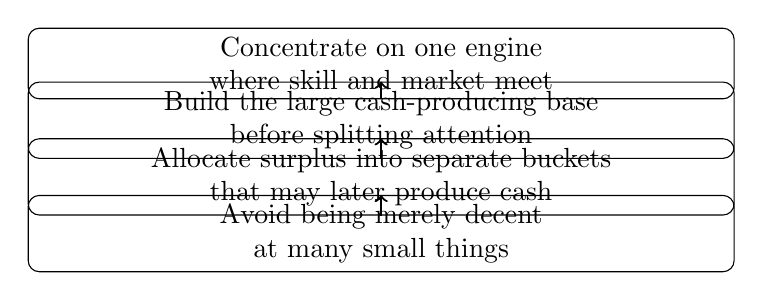
\begin{tikzpicture}[
  node distance=0.72cm,
  box/.style={draw, rounded corners, align=center, text width=0.72\linewidth, minimum height=0.75cm},
  arrow/.style={->, thick}
]
\node[box] (focus) {Concentrate on one engine\\where skill and market meet};
\node[box, below of=focus] (pile) {Build the large cash-producing base\\before splitting attention};
\node[box, below of=pile] (allocate) {Allocate surplus into separate buckets\\that may later produce cash};
\node[box, below of=allocate] (avoid) {Avoid being merely decent\\at many small things};
\draw[arrow] (focus) -- (pile);
\draw[arrow] (pile) -- (allocate);
\draw[arrow] (allocate) -- (avoid);
\end{tikzpicture}
\caption{The interview's concentration-before-diversification mechanism, redrawn as a narrow flow for pocket layout.}
\end{figure}

The mechanism can be written as a sequence:
\begin{align}
\text{skill concentration} &\longrightarrow \text{market traction},\\
\text{market traction} &\longrightarrow \text{large cash-producing base},\\
\text{large base} &\longrightarrow \{A_1,A_2,\ldots,A_n\},
\end{align}
where \(A_i\) are later allocations. The important point is order. Diversification is not denied forever; it is delayed until there is something meaningful to diversify.

\section{Attention As Distribution}

The interviewer next asks about content. Mitt has a social audience, but he does not present it as fame for its own sake. He gives specific figures:
\begin{equation}
F_{\text{TikTok}} \approx 145{,}000,
\qquad
F_{\text{Instagram}} \approx 25{,}000.
\end{equation}
He then gives the operational payoff. In a company meeting, he says roughly \(30\%\) to \(40\%\) of new starters reported that they had been following him before they saw the job.

\begin{equation}
P(\text{new starter followed Grant first})
\approx 0.30\text{--}0.40.
\end{equation}

The mechanism is not merely audience size. It is a path from public teaching to trust, from trust to recruiting, and from recruiting to capability inside the company. He also says the visibility helped him get appearances on Fox Business and other opportunities that might not have come even if the company had been larger without his public presence.

A concise model is
\begin{align}
\text{free information} &\longrightarrow \text{personal brand},\\
\text{personal brand} &\longrightarrow \text{credibility},\\
\text{credibility} &\longrightarrow \text{recruiting and opportunities}.
\end{align}

The style of the answer matters. He is not saying that every business owner must become a celebrity. He is saying that visible helpfulness can become a distribution channel for people, trust, and attention.

\section{Risk, Sales, And Repeatable Skill}

The risk section begins with the blunt claim that risk-taking is everything, then immediately qualifies it: there are times to be risk-on and risk-off, and one must prepare for rainy days. The deeper claim is that the best risk is a bet on a repeatable capability.

Mitt's Ferrari line gives the time preference: he would rather enjoy the results at 27, 35, or 40 than defer all reward until 75. The Sahara Desert line gives the portability claim: if his brain and abilities still worked, he believes he could rebuild in half the time because he now knows the process.

We can write the underlying update rule as
\begin{equation}
S_{t+1}=S_t+\Delta S(\text{repetition},\text{feedback},\text{rejection},\text{adaptation}),
\end{equation}
where \(S_t\) denotes the operator's practical skill at time \(t\). This is not a formal empirical law. It is a faithful mathematical shorthand for the sales argument that follows.

\paragraph{Worked example.}
Suppose a young salesperson begins with a baseline skill \(S_0\). Each hard sales interaction contributes a small increment \(a\), but only if the person receives feedback and returns to the next interaction with the same standard of delivery. After \(n\) serious repetitions, the simplest linear model is
\begin{equation}
S_n = S_0 + na.
\end{equation}
If emotional carryover causes the person to degrade after rejection, the effective increment is smaller:
\begin{equation}
S_n = S_0 + n(a-\ell),
\end{equation}
where \(\ell\) is the loss from poor emotional recovery. The interview's sales lesson is that the operator must keep \(a\) positive through rejection: no, no, cursing, screaming, cold calls, doors, and difficult customers.

That is why the sales story belongs next to the risk story. ``You can't Google experience'' is not a throwaway line. It is the mechanism by which self-trust becomes less imaginary. At 18 or 19, Mitt says, he was selling DirecTV in Walmart to people who were tired, irritated, or buying groceries. The repeated exposure trained communication across age, background, mood, and resistance.

\section{Scaling Means People Doing Fundamentals}

The scaling question begins with a concrete number: Mitt Group was closing solar deals in 17 states.
\begin{equation}
N_{\text{states}}=17.
\end{equation}
The interviewer asks how to move from six or seven figures toward eight figures. Mitt's definition is the cleanest definition-like sentence in the interview: scaling is doing the little things right at scale.

\begin{definition}
In this chapter, \emph{scale} means that correct fundamentals are executed by many capable people without the founder personally supervising every action.
\end{definition}

\subsection{Question \& Answer}

\paragraph{Question.}
Why are CRM systems, technology, and one smart hire not enough to scale a company?

\paragraph{Answer.}
Mitt allows that tools may help, but he gives them a limited effect. They might improve the business by \(10\%\) or \(20\%\), but he says they will not double, triple, or quadruple revenue by themselves:
\begin{equation}
\Delta R_{\text{tools}}\approx 10\%\text{--}20\%,
\qquad
\Delta R_{\text{tools}}\not\approx 2R,3R,4R.
\end{equation}
The larger multiplier comes from people who know what they are doing in specific areas and can operate effectively without the founder doing everything for them.

\begin{figure}
\centering
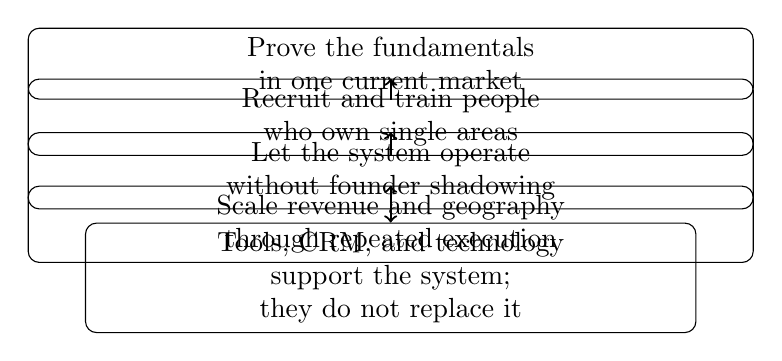
\begin{tikzpicture}[
  node distance=0.68cm,
  box/.style={draw, rounded corners, align=center, text width=0.74\linewidth, minimum height=0.72cm},
  side/.style={draw, rounded corners, align=center, text width=0.62\linewidth, minimum height=0.6cm},
  arrow/.style={->, thick}
]
\node[box] (local) {Prove the fundamentals\\in one current market};
\node[box, below of=local] (people) {Recruit and train people\\who own single areas};
\node[box, below of=people] (delegate) {Let the system operate\\without founder shadowing};
\node[box, below of=delegate] (scale) {Scale revenue and geography\\through repeated execution};
\node[side, below of=scale] (tools) {Tools, CRM, and technology\\support the system;\\they do not replace it};
\draw[arrow] (local) -- (people);
\draw[arrow] (people) -- (delegate);
\draw[arrow] (delegate) -- (scale);
\draw[arrow] (scale) -- (tools);
\end{tikzpicture}
\caption{Scaling in the interview: fundamentals first, then people, then delegation, with tools as secondary support.}
\end{figure}

This also explains the warning against expanding too early. Before we ask whether to move to Europe, another state, or another city, we must ask whether the current place is actually being conquered.

\section{Energy, Industry Choice, And Team Filters}

The burnout answer turns the chapter inward again. Mitt says burnout happens when we do not control energy and emotions. The model is simple: the day begins with a finite stock of energy, and each communication, interaction, and decision draws from it.

A cautious reconstruction is
\begin{equation}
E_{\text{remaining}}
=
E_{\text{day}}
-\sum_{i=1}^{n} c_i
-L_{\text{emotion}},
\end{equation}
where \(c_i\) is the cost of the \(i\)-th interaction or decision, and \(L_{\text{emotion}}\) is the extra loss from anger, frustration, or emotional carryover. Mitt's example is direct: if an appointment goes badly and we spend energy being upset, that waste affects the next appointment.

The rule is not passive calm. It is operational conservation. Saying no matters because it protects the finite resource:
\begin{equation}
\text{Good no} \longrightarrow \text{less wasted energy} \longrightarrow \text{better next action}.
\end{equation}

The interview then asks why solar. Mitt says that during his short time in college, around 2014 to 2016, he looked for industries likely to be bigger in twenty years: technology, artificial intelligence, robotics, renewable energy, crypto. He did not claim mastery at the start. He looked for a door into an expanding field and a place where fewer of his peers were going.

The final hiring discussion gives the people filter. Talent is not enough. School is not enough. Referrals are not enough. The non-negotiables are coachability, humility, and persistence. He adds one more harsh observation: people with easy fallback plans often do not have the same necessity. The person who has to make it, he says, will find a way.

\begin{table}
\centering
\begin{tabular}{p{0.30\linewidth}p{0.58\linewidth}}
Filter & Interview meaning \\
Coachable & Can absorb the company's way of operating rather than merely arriving with talent \\
Humble & Can be corrected without turning correction into identity threat \\
Persistent & Continues through rejection, difficulty, and repetition \\
No easy fallback & Has enough necessity to keep going when the work becomes uncomfortable \\
\end{tabular}
\caption{Mitt's hiring filters, stated as operating traits rather than credentials.}
\end{table}

\section{Summary}

The chapter's argument is a sequence. First, the market chooses, so age is not the central variable. Second, the base rates of business ownership are poor enough that starting a company needs more than romance. Third, Mitt's reason for starting was necessity under prepared conditions. Fourth, wealth creation came from concentration before diversification. Fifth, social media mattered because it created distribution, recruiting, and credibility. Sixth, risk became rational only because skill had become repeatable through sales experience. Seventh, scale meant people executing fundamentals without founder dependence. Finally, burnout, industry selection, and hiring all returned to the same operating discipline: protect energy, choose expanding fields, and find people whose traits survive pressure.